\section{System \"Ubersicht}

\subsection{Komponentendiagramm}

\begin{figure}[H]
  \centering
  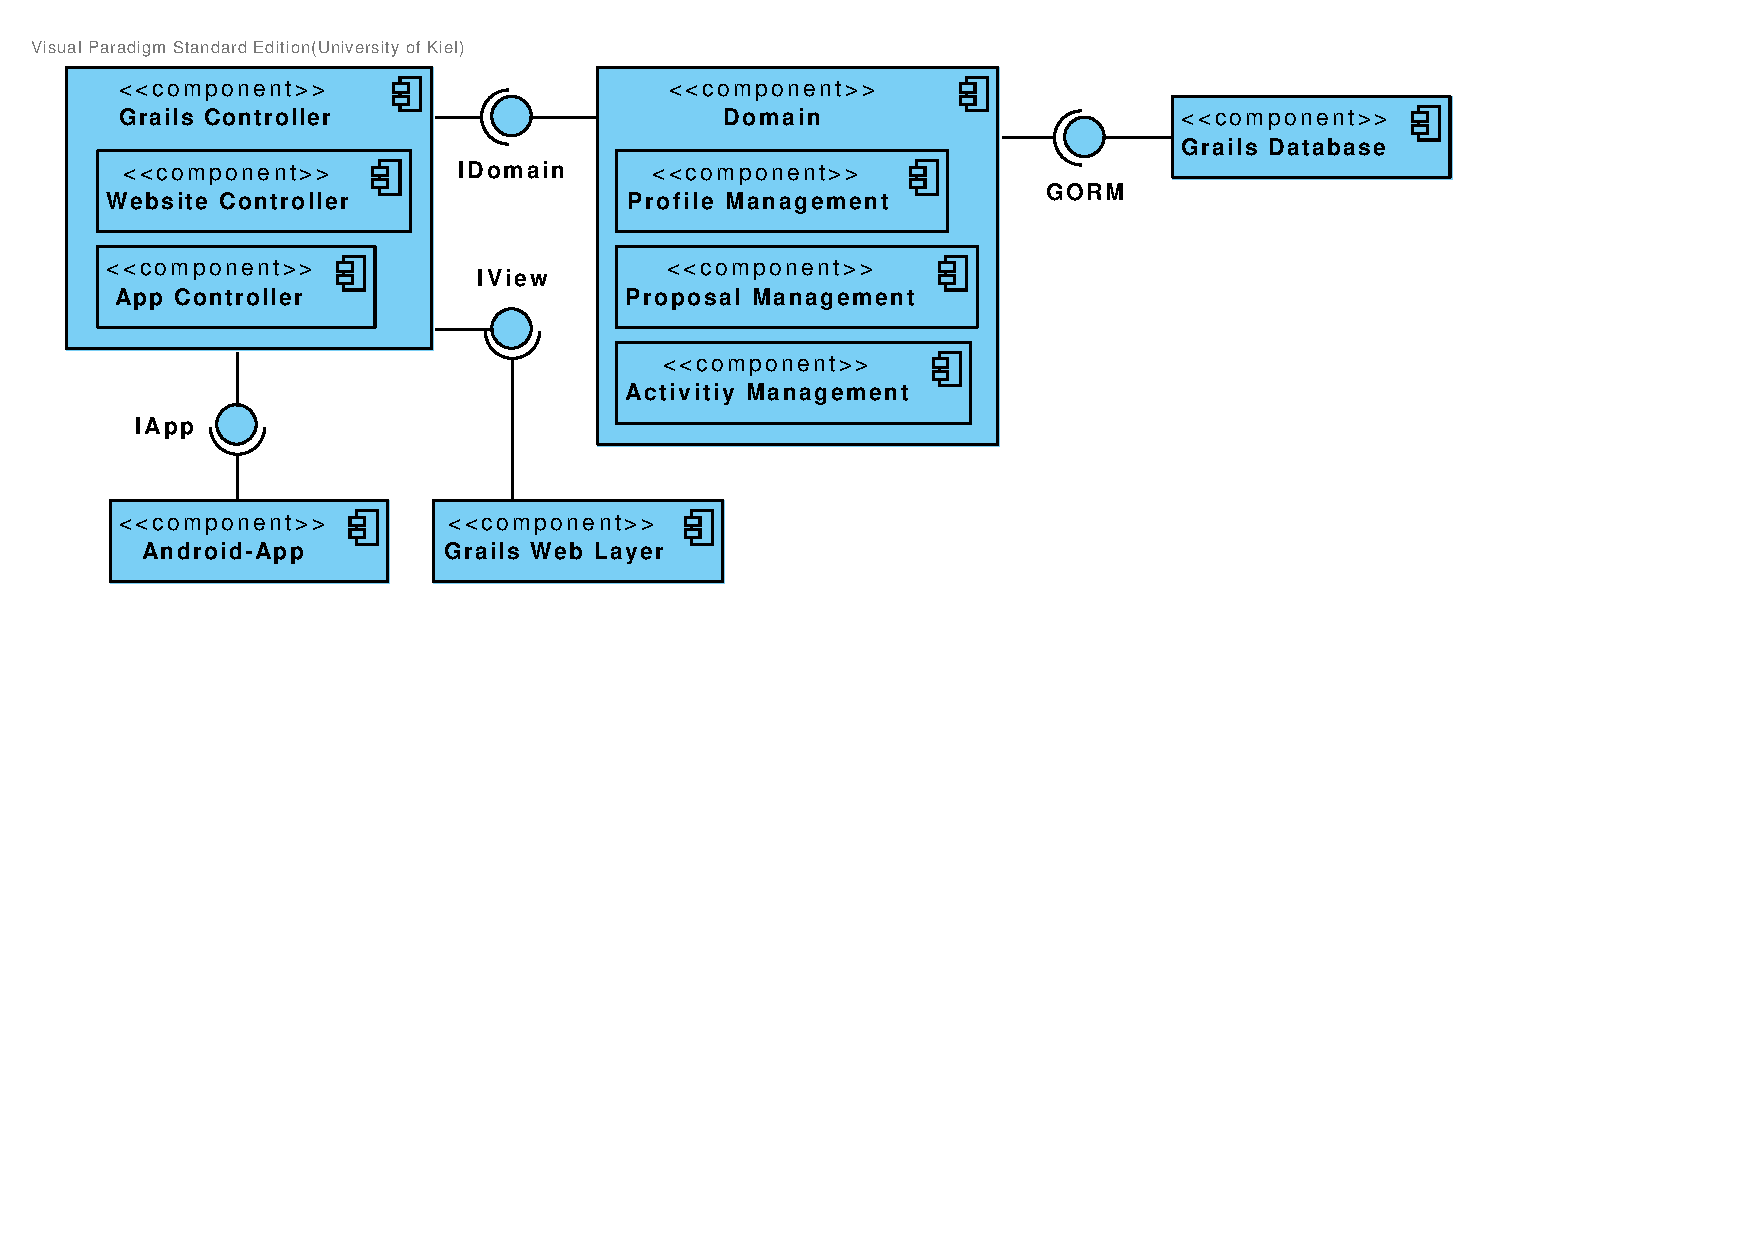
\includegraphics[width=\textwidth, trim=1cm 11cm 4cm 1cm, clip]{gfx/component_diagram}
  \caption{Komponentendiagramm}
\end{figure}

\paragraph{Grails Database} Die Grails Database Komponente ist die zentrale Datenbank, die auf dem Server liegt und s\"amtliche Daten enth\"alt, auf die, \"uber das durch \emph{Grail's Object Relational Mapping} (GORM) bereitgestellte Interface, zugegriffen werden kann.

\paragraph{Domain} Die Domain Komponente ist die Modell
Repr\"asentation der Daten in der Datenbank. Der Zugriff erfolgt
\"uber das IDomain Interface. Die Domain Komponenten ist unterteilt in
die Subkomponenten \emph{Profile Management}, \emph{Proposal
  Management} und \emph{Activity Management}. Das Profile Management
ist zuständig für die Verwaltung der Modellrepräsentation von Team-
und Benutzerprofilen. Das Proposal Managment ist zuständig für die
Verwaltung der Modellrepräsentation von (Aktivitäts-) Vorschlägen. Die
Komponente Activity Management ist zuständig für die Verwaltung der Modellrepräsentation von Aktivitäten.

\paragraph{Grails Web Layer} Die Grails Web Layer Komponente kommuniziert mit dem Grails Controller \"uber das IView Interface und stellt die GSP Dateien zur Verf\"ugung, die das Layout der Webseite spezifizieren.

\paragraph{Grails Controller} Die Controller Komponente besteht aus den einzelnen Controllern f\"ur Webseite und Android App und ist zust\"andig f\"ur die Verarbeitung s\"amtlicher Daten und Anfragen, die \"uber die IApp, IDomain und IView Schnittstellen kommuniziert werden.

\paragraph{Android App} Die Android App, dient in erster Linie zur Repr\"asentation der Daten vom Server auf Mobilger\"aten. Sie kommuniziert \"uber das IApp Interface mit dem Controller.

\subsection{Verteilungsdiagramm}

\begin{figure}[H]
  \centering
  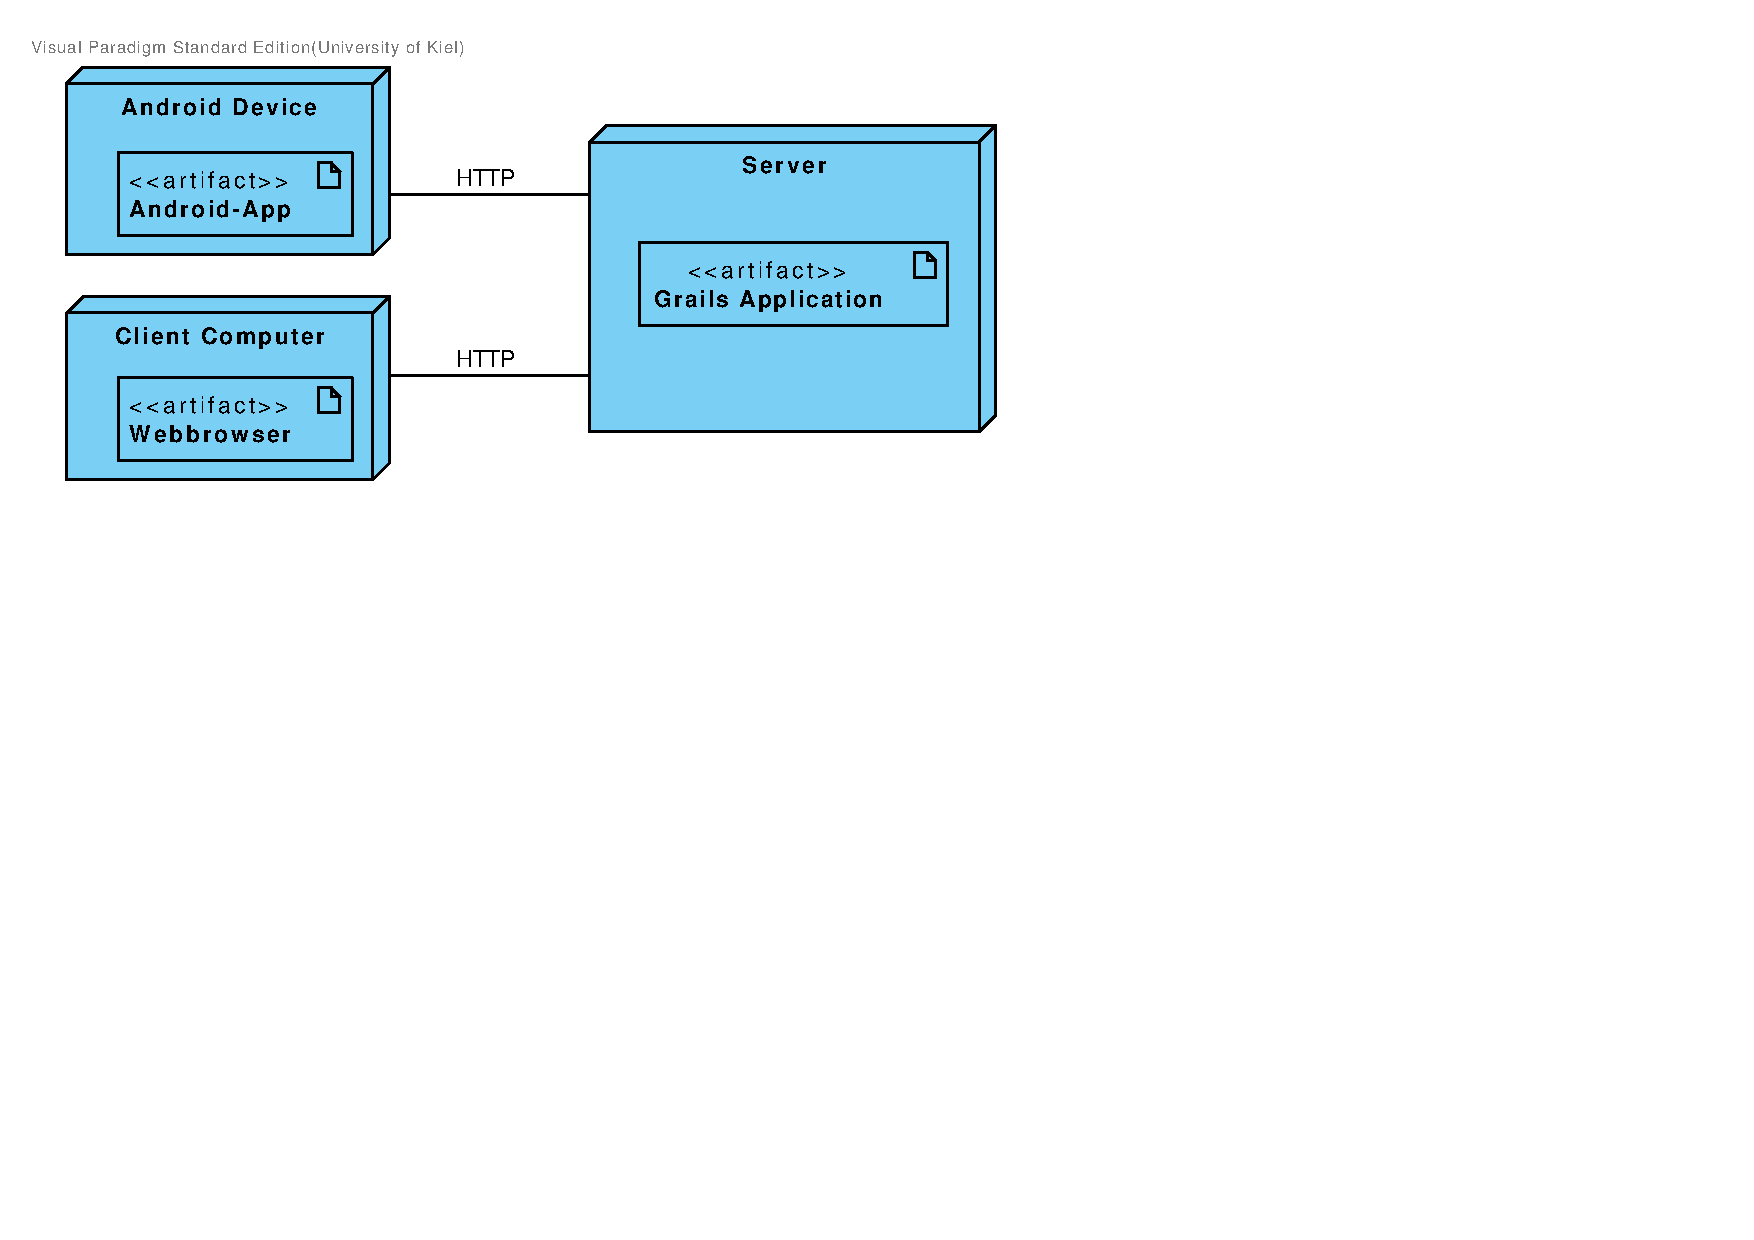
\includegraphics[width=\textwidth, trim=1cm 12cm 12cm 1cm, clip]{gfx/deployment_diagram}
  \caption{Verteilungsdiagramm}
\end{figure}

\subsubsection{Android Device}
Das Android Device ist das Arbeitswerkzeug für die Benutzer. Auf dem
Gerät ist eine native Android-Applikation installiert, mit der Daten
eingegeben und abgerufen werden können. Der Benutzer muss bereits
registriert sein, um die Applikation nutzen zu können.

\subsubsection{Client Computer}
Benutzer können mit Hilfe eines Computers über einen Webbrowser auf eine Webseite zugreifen, welche, nach erfolgreichem einloggen, verschiedene Funktionen zur Aktivitäts- und Profilverwaltung anbietet.Des Weiteren können hier auch anonymisierte Statistiken angezeigt und diese statistischen Daten exportiert werden.

\subsubsection{Server}
Der Server stellt die eben erwähnte Webseite bereit. Hier werden gegebenenfalls Datenanfragen von den Android-Geräten verarbeitet.

\subsection{Paketdiagramm}
Sowohl die Grails-Webanwendung als auch die Android-App befindet sich einem Paket \emph{de.unikiel.klik}.

\subsubsection{Grails Anwendung}

\begin{figure}[H]
  \centering
  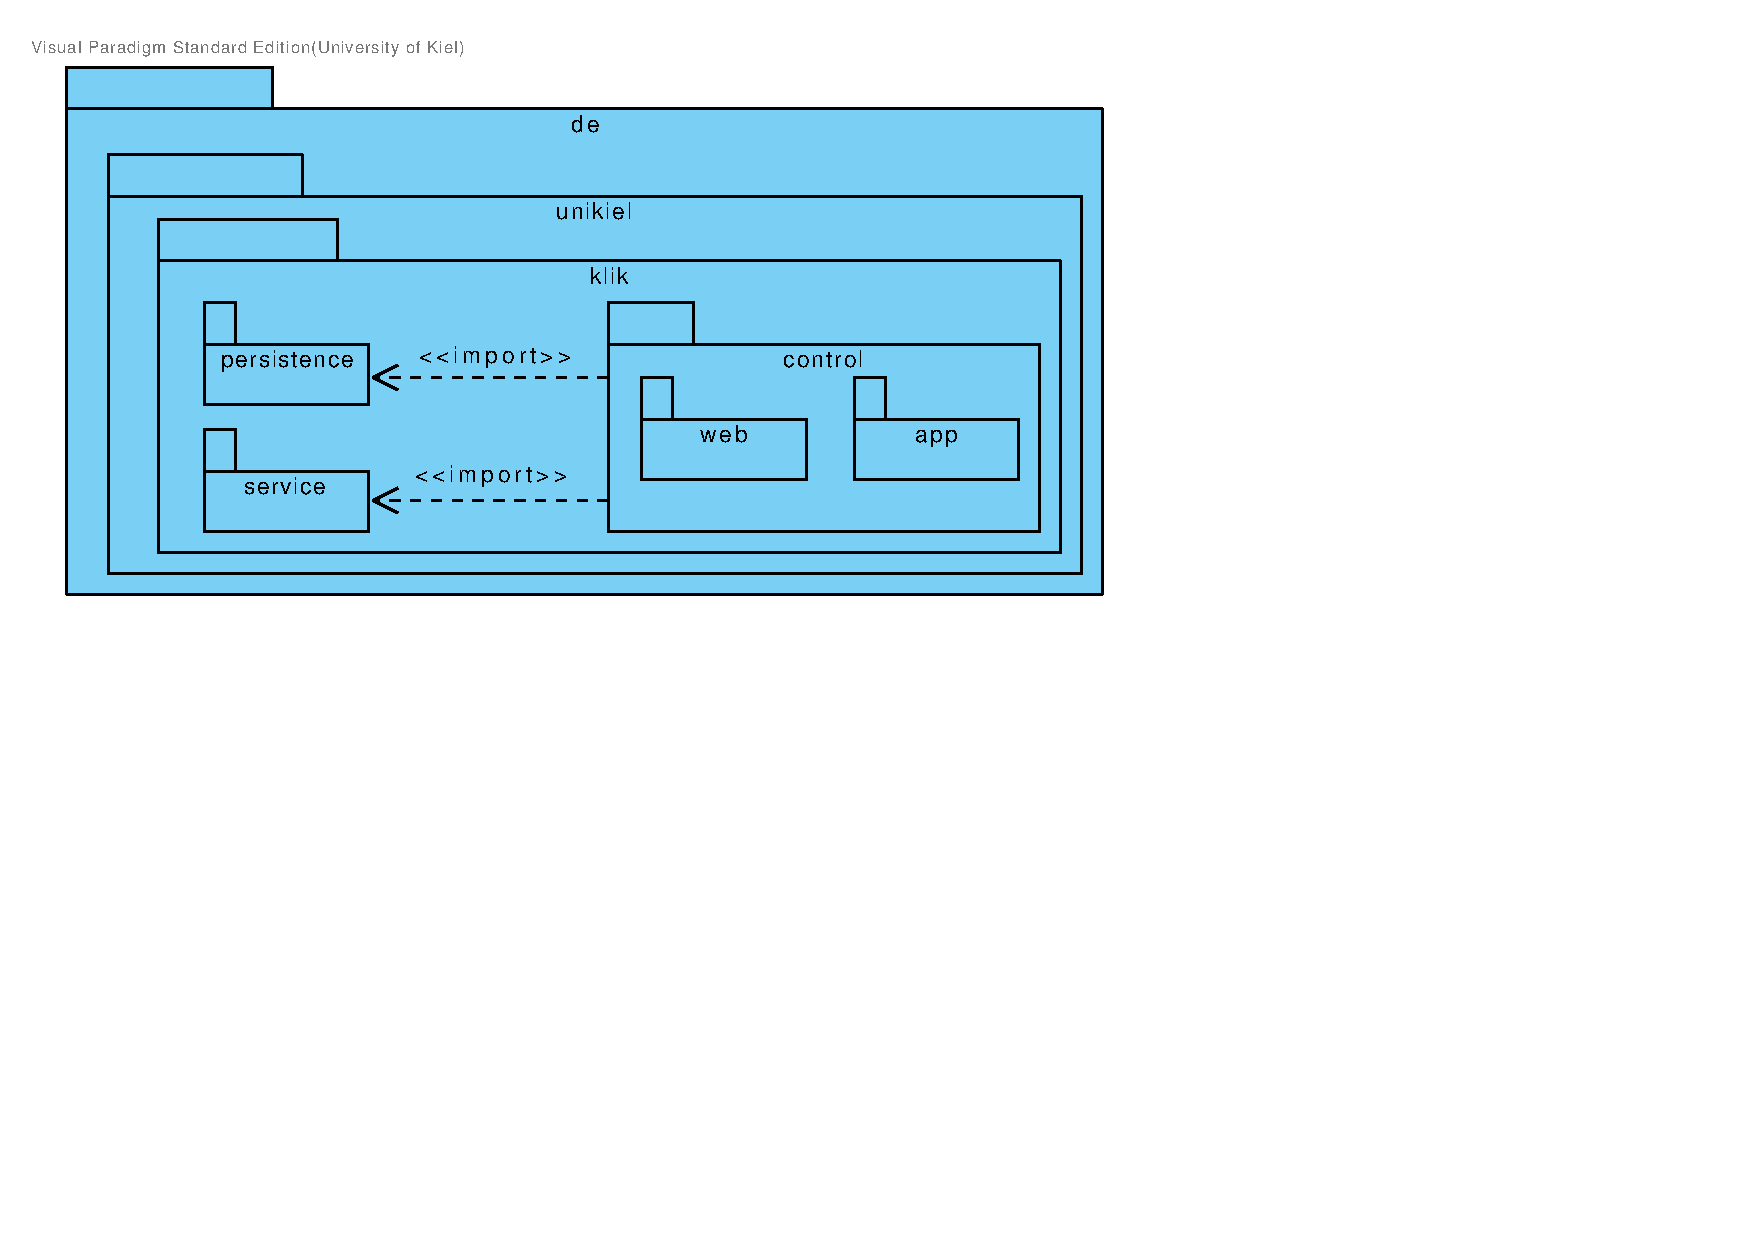
\includegraphics[width=\textwidth, trim=1cm 10cm 11cm 1cm, clip]{gfx/package_diagram}
  \caption{Pakete der Grails Anwendung}
\end{figure}

%TODO Beschreibung der Packages
\paragraph{persistence} In diesem Paket befinden sich die Klassen, die für die Datenhaltung zuständig sind.
\paragraph{control} In diesem Paket befinden sich die Klassen, die für die Klassen, die Serveranfragen entgegennehmen und diese verarbeiten.
\paragraph{control.web} Die Klassen, die Anfragen von der Website entgegen nehmen und diese verarbeiten, befinden sich in diesem Paket.
\paragraph{control.app} Die Klassen, die Anfragen von der Android-App entgegen nehmen und diese verarbeiten, befinden sich in diesem Paket.
\paragraph{service} In diesem Paket befinden sich Klassen, die als Bindeglied zwischen dem \emph{control}- und dem \emph{persistence}-Paket stehen. Dies sind zum einem einen Klassen, die Änderungen auf den Daten vornehmen, und zum anderen Klassen, die Methoden bereitstellen, die von verschiedenen \emph{[control]}-Klassen verwendet werden.

\subsubsection{Android App}

\begin{figure}[H]
  \centering
  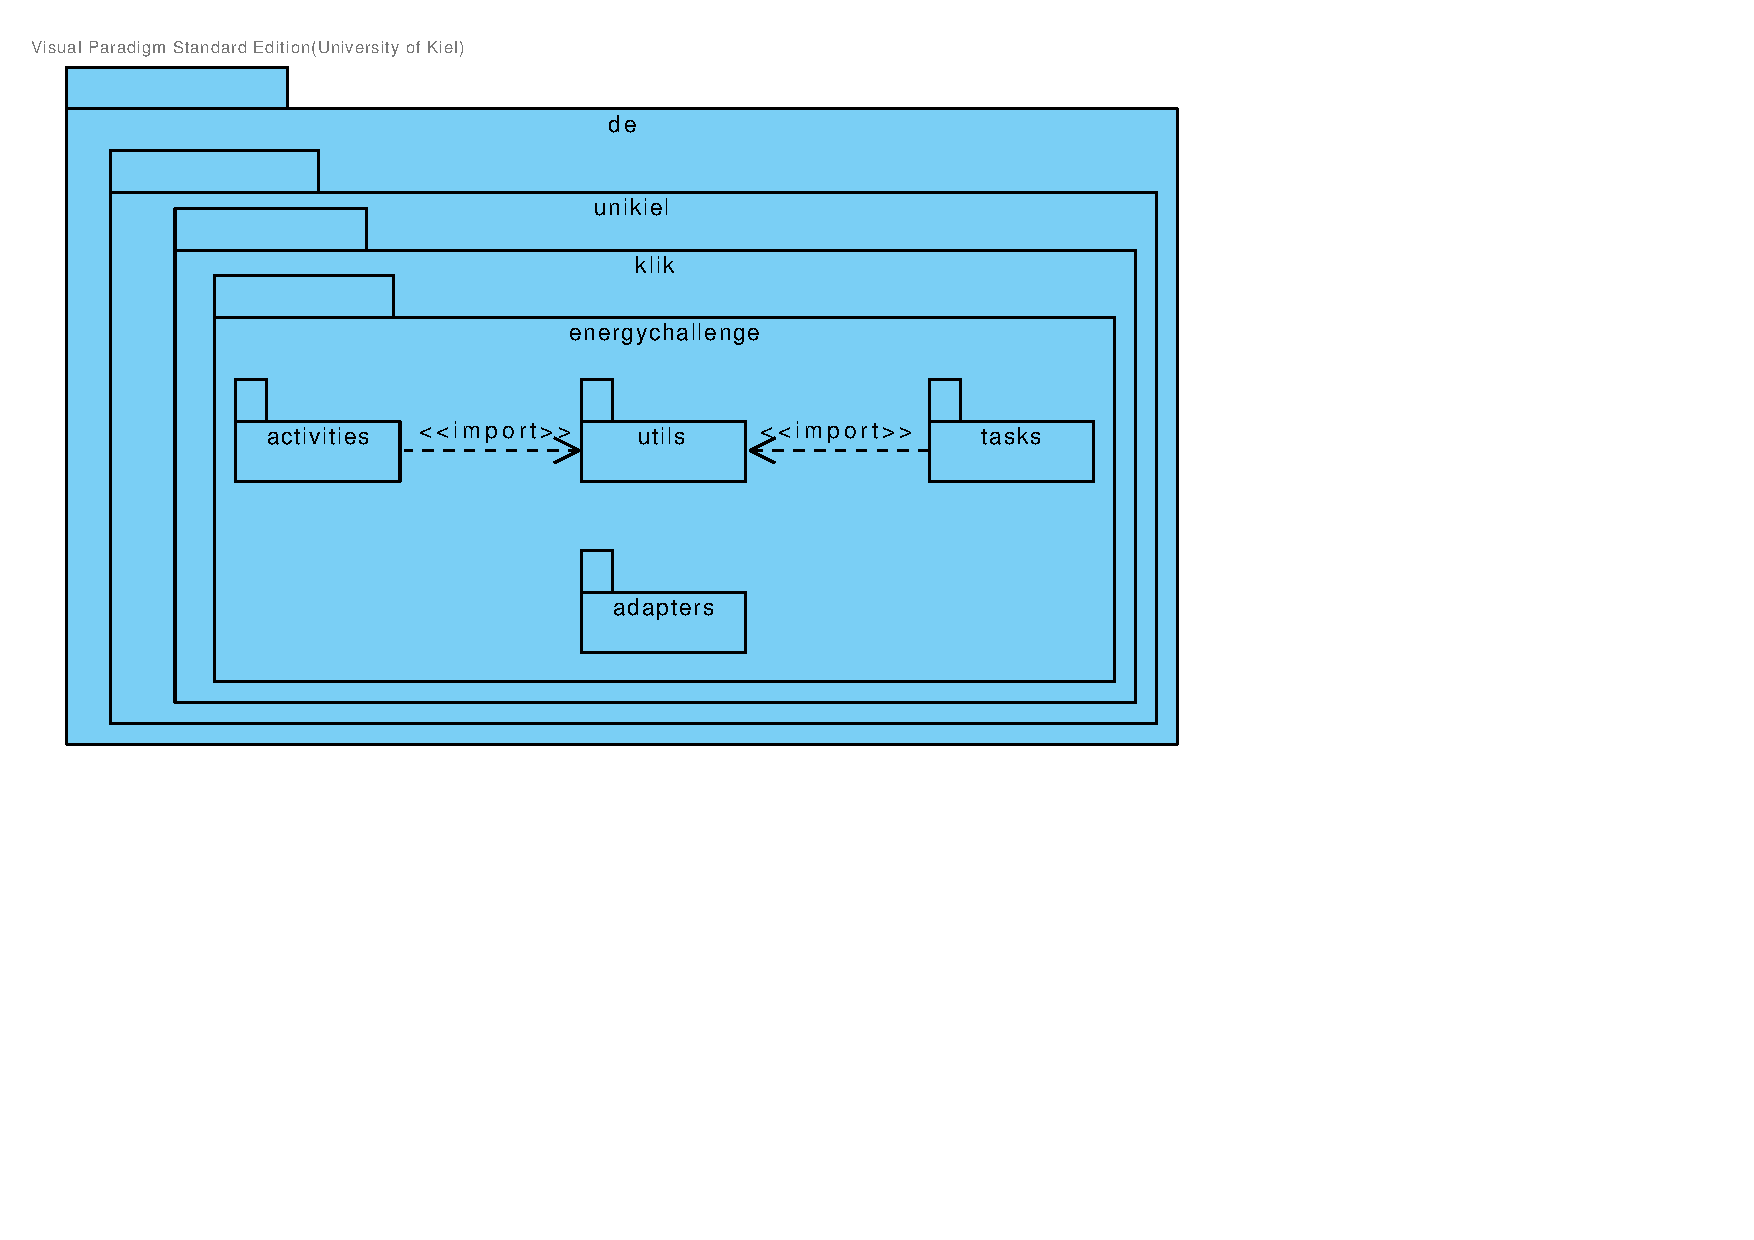
\includegraphics[width=\textwidth, trim=1cm 7cm 9cm 1cm, clip]{gfx/app_package_diagram}
  \caption{Pakete der Android App}
\end{figure}

%TODO Beschreibung der Pakete der Android App